\section{Experimental Evaluation}
\label{sec:results}
% Numerical sources: the main report Tables 1 and 3 and Section 4.11.
% Saved views: comparison and design_comparison; statistics are unchanged.
% Mechanism interventions use their runtime-matched local standards.

\newcommand{\HadMainTable}{%
\begin{table*}[!t]
\centering\footnotesize
\setlength{\tabcolsep}{5pt}
\caption{Eight-method comparison of target protection: damage $D\downarrow$, mean $\pm$ sample SD across three training seeds (Rule: scene SD). Each configuration uses 300 common scenes; configurations are equally weighted. QMIX denotes the entity-attention adaptation. Bold: lowest mean.}
\label{tab:had-main}
\begin{tabular*}{\textwidth}{@{\extracolsep{\fill}}lrrrr@{}}
\toprule
Method & ID & $K$-OOD & $N$-OOD & Joint OOD \\
\midrule
\textbf{LEAF} & $\mathbf{0.405\pm0.097}$ & $\mathbf{0.996\pm0.233}$ & $\mathbf{0.575\pm0.235}$ & $\mathbf{1.097\pm0.105}$ \\
REFIL & $0.715\pm0.049$ & $1.796\pm0.304$ & $2.209\pm0.277$ & $3.308\pm0.303$ \\
ALMA & $1.326\pm0.193$ & $3.022\pm0.344$ & $3.605\pm0.742$ & $5.375\pm1.036$ \\
TransfQMix$^{\ddagger}$ & $1.529\pm0.283$ & $3.953\pm0.495$ & $4.024\pm0.968$ & $6.630\pm1.203$ \\
DCG & $2.028\pm0.437$ & $5.839\pm1.920$ & $5.021\pm2.658$ & $8.092\pm3.909$ \\
SPECTra$^{\ddagger}$ & $2.485\pm0.209$ & $6.743\pm0.528$ & $5.049\pm0.589$ & $9.838\pm0.490$ \\
Rule$^{\dagger}$ & $1.462\pm0.717$ & $3.212\pm1.126$ & $1.545\pm0.881$ & $3.060\pm0.976$ \\
QMIX & $2.318\pm1.431$ & $5.009\pm2.497$ & $5.139\pm3.111$ & $7.415\pm3.970$ \\
\bottomrule
\end{tabular*}
\par\vspace{2pt}\parbox{\textwidth}{\footnotesize
$\dagger$ Rule has no training seeds; its SD is across the 300 scene seeds after averaging configurations within each scene. Other SDs describe variation across trained models. $\ddagger$ Updated baselines align entity inputs and sampling controls while retaining their method-specific optimizer and TD settings.}
\end{table*}}

\newcommand{\HadCoreAblationTable}{%
\begin{table*}[!t]
\centering\footnotesize
\setlength{\tabcolsep}{3pt}
\caption{Historical architecture design comparisons: damage $D\downarrow$, mean $\pm$ sample SD across three training seeds, under the formal evaluation of Table~\ref{tab:had-main}. The middle column states the principal module change. C: context constructor; Q: current-self query; F: stage fusion; H: host integration. Temporal GRU is retained by every trained variant. Bold: lowest mean.}
\label{tab:had-core-ablation}
\begin{tabular*}{\textwidth}{@{\extracolsep{\fill}}lp{0.30\textwidth}rrrr@{}}
\toprule
Variant & Module / change & ID & $K$-OOD & $N$-OOD & Joint OOD \\
\midrule
\textbf{LEAF} & Complete architecture & $\mathbf{0.405\pm0.097}$ & $\mathbf{0.996\pm0.233}$ & $\mathbf{0.575\pm0.235}$ & $\mathbf{1.097\pm0.105}$ \\
Direct read & C: bypass updates; read $H^{(0)}$ & $0.928\pm0.210$ & $1.958\pm0.457$ & $2.020\pm0.446$ & $3.196\pm0.687$ \\
Memory query & Q: add stopped-gradient history & $0.527\pm0.227$ & $1.529\pm0.734$ & $0.998\pm0.621$ & $1.946\pm1.229$ \\
Last read & F: use only the exit's final read & $0.434\pm0.083$ & $1.020\pm0.100$ & $0.652\pm0.160$ & $1.269\pm0.202$ \\
No host & H: remove REFIL attention, imagined groups, and auxiliary loss & $0.510\pm0.138$ & $1.768\pm0.621$ & $1.263\pm0.653$ & $2.319\pm0.889$ \\
\bottomrule
\end{tabular*}
\par\vspace{2pt}\parbox{\textwidth}{\footnotesize
All four historical variants use stopped-gradient history queries; LEAF uses a current-self query. Direct read, Last read, and No host therefore differ in query placement as well as the listed module. No host retains the self-projection residual and temporal memory. Depth-training and parameter-sharing comparisons appear in Table~\ref{tab:had-supplement}.}
\end{table*}}

\newcommand{\HadMechanismTable}{%
\begin{table*}[!t]
\centering\footnotesize
\setlength{\tabcolsep}{3pt}
\caption{Frozen-policy mechanism interventions: paired damage increase $\Delta D=D_{\mathrm{intervention}}-D_{\mathrm{local\ standard}}$, mean $\pm$ sample SD across three models. Each model uses ten scenes per configuration. Positive values indicate worse protection. These interventions probe learned policy dependence, not independently retrained removals.}
\label{tab:leaf-mechanism}
\begin{tabular*}{\textwidth}{@{\extracolsep{\fill}}llrrr@{}}
\toprule
Intervention & Path probed & $(10,10,2)$ & $(50,50,2)$ & $(30,30,12)$ \\
\midrule
Read initial $H^{(0)}$ & H1: constructed context & $7.556\pm1.365$ & $18.962\pm5.828$ & $32.968\pm8.447$ \\
Zero relational residual & H1: relational feature path & $5.950\pm1.525$ & $13.695\pm6.899$ & $18.788\pm1.144$ \\
Force final read & H2: intermediate-stage fusion & $6.728\pm3.186$ & $19.937\pm12.955$ & $25.558\pm16.414$ \\
Reset Temporal GRU & H2: downstream temporal memory & $1.423\pm0.760$ & $1.294\pm0.869$ & $1.655\pm2.563$ \\
\bottomrule
\end{tabular*}
\par\vspace{2pt}\parbox{\textwidth}{\footnotesize
The $H^{(0)}$ bypass uses SkyHAD 3.0.0; the other interventions use the archived HAD-workbench 2.1.0 runtime. Each difference is paired with its corresponding local standard, separately from the formal 300-scene evaluation.}
\end{table*}}

\newcommand{\HadSupplementTable}{%
\begin{table*}[!t]
\centering\footnotesize
\setlength{\tabcolsep}{3pt}
\caption{Supplementary design and capacity controls: damage $D\downarrow$, mean $\pm$ sample SD across three training seeds. Each row is separately trained with the same physical-step budget and uses the formal evaluation of Table~\ref{tab:had-main}. These controls examine training depth, parameter sharing, and host capacity; they are distinct from the frozen exits in Fig.~\ref{fig:mechanism}(c). Bold: lowest mean.}
\label{tab:had-supplement}
\begin{tabular*}{\textwidth}{@{\extracolsep{\fill}}lp{0.30\textwidth}rrrr@{}}
\toprule
Method / variant & Design or capacity change & ID & $K$-OOD & $N$-OOD & Joint OOD \\
\midrule
\textbf{LEAF} & Shared updates; train R1--R4 & $\mathbf{0.405\pm0.097}$ & $\mathbf{0.996\pm0.233}$ & $0.575\pm0.235$ & $\mathbf{1.097\pm0.105}$ \\
One round & Train and execute R1 only & $0.609\pm0.272$ & $1.203\pm0.402$ & $1.355\pm0.884$ & $2.157\pm1.006$ \\
Fixed depth & Train at R4 throughout & $0.407\pm0.204$ & $1.004\pm0.665$ & $0.659\pm0.184$ & $1.265\pm0.230$ \\
Unshared rounds & Independent update blocks per round & $0.476\pm0.183$ & $1.127\pm0.157$ & $\mathbf{0.543\pm0.156}$ & $1.232\pm0.253$ \\
REFIL-matched & Enlarge host to 176,393 actor parameters & $0.914\pm0.165$ & $2.493\pm0.280$ & $2.269\pm0.312$ & $4.170\pm0.760$ \\
\bottomrule
\end{tabular*}
\par\vspace{2pt}\parbox{\textwidth}{\footnotesize
One round, Fixed depth, and Unshared rounds retain stopped-gradient history queries, unlike LEAF. Single-round fusion is trivial. Unshared rounds also increases parameter count. The comparisons with LEAF are not single-factor changes, and equal physical-step budgets do not imply equal computation budgets.}
\end{table*}}


\noindent\textbf{Setup.}
We evaluate the planar HAD target-protection task~\cite{skyhad2026}, using public entity-state observations, a fixed reactive--rush attacker, and at most 100 physical steps per episode. Training independently samples balanced teams $N_R=N_B=N\in\{4,6,8,10\}$ and target counts $K\in\{1,2,3\}$. Each learned method uses three training seeds and $10^6$ physical environment steps per seed. LEAF uses width 64, four attention heads, learning rate $5\times10^{-4}$, discount 0.99, batch size 32, and replay capacity 5000. It samples R1--R4 during training and uses R4 for the formal comparison. All evaluations use the final budget-complete checkpoints with frozen parameters.

In-distribution (ID) evaluation contains $(4,4,2)$, $(6,6,2)$, $(8,8,2)$, and $(10,10,3)$. Target-count extrapolation ($K$-OOD) uses $(10,10,K)$ with $K=4,6,9,12$. Team-size extrapolation ($N$-OOD) uses $(N,N,2)$ with $N=15,20,25,30,40,50$. Joint OOD combines $N=15,20,30$ with $K=4,6$, and adds $(30,30,9)$ and $(30,30,12)$. Two extra configurations, $(5,5,2)$ and $(10,10,2)$, complete the 24-configuration matrix. Every configuration uses 300 common initial scenes, seeds 9000--9299. Transfer is zero-shot: neither the policy parameters nor the entity encoder are adapted to these deployment populations. The label R1 denotes execution depth $L=1$, and similarly for the other exits.

\noindent\textbf{Metrics and uncertainty.}
The primary metric is cumulative target damage $D\downarrow$, with unshaped episode reward $R=-D$. Damage is not capped by initial target health and is not a win rate. Where recorded, we also report friendly-collision mortality $C$ (defenders killed by friendly collisions divided by initial $N_R$), attacker interception $I$, and the fraction of episodes with any target damage $P$. The updated SPECTra and TransfQMix final evaluations record damage but not these protection diagnostics. Results first average scenes within each trained model and configuration, then weight group configurations equally. The reported mean $\pm$ sample SD describes variation across three trained models~\cite{agarwal2021rliable}; Rule instead uses scene-seed SD. Validation has 50 checkpoints, each evaluating four ID configurations on 25 fixed scenes distinct from the formal pool. Curves align checkpoint indices, use actual mean environment-step counts, and show unsmoothed model means and sample SD.

\subsection{Comparison Across Deployment Populations}
\label{subsec:comparison}
The comparison in Table~\ref{tab:had-main} and Fig.~\ref{fig:comparison} includes LEAF, REFIL~\cite{iqbal2021refil}, ALMA~\cite{iqbal2022alma}, TransfQMix~\cite{transfqmix2023}, DCG~\cite{boehmer2020dcg}, SPECTra~\cite{park2026spectra}, Rule, and QMIX~\cite{rashid2018qmix}. Here QMIX denotes the documented entity-attention adaptation. The updated SPECTra and TransfQMix runs use 19-dimensional entity inputs, including the previous action, consistently in actor and mixer; both use eight parallel collectors and eight learner updates per collection. Their own optimizer and TD settings are retained: Adam at $10^{-3}$, TD($\lambda$) with $\lambda=0.6$, and half-MSE loss. All learned methods use equal physical-step budgets. This aligns inputs and sampling controls, not every training hyperparameter; the historical LEAF design comparisons provide closer architectural contrasts, with query differences noted below.

LEAF has the lowest group mean damage in all four groups. Relative to REFIL, $D$ decreases by 0.310, 0.800, 1.635, and 2.211 in ID, $K$-OOD, $N$-OOD, and Joint OOD; all three training-seed comparisons favor LEAF in each group. The larger differences when teams and targets grow together support the intended use of attacker--target--teammate context: a policy learned in small engagements continues to protect assets as the entity set expands.

Figure~\ref{fig:comparison} connects validation to deployment for the same eight methods. At checkpoint 10, around 0.2M physical steps, LEAF's validation damage is $2.046\pm0.028$, versus REFIL's $4.429\pm0.284$; the final values are $0.373\pm0.066$ and $0.738\pm0.122$. These observations describe the fixed ID validation pool, while the extrapolation panels track the frozen policies as population size changes.

Among learned comparators with recorded final protection diagnostics, LEAF has lower mean friendly-collision mortality in all four groups. This comparison excludes the updated SPECTra and TransfQMix runs. Rule has lower $C$ in $N$-OOD and Joint OOD: $5.70\pm3.30\%$ and $4.48\pm2.44\%$, compared with LEAF's $6.29\pm1.32\%$ and $4.97\pm1.26\%$. Its target damage is higher in both groups. Conserving defenders and protecting targets therefore remain distinct outcomes; the latter is the primary objective.

\HadMainTable

\begin{figure*}[!t]
\centering
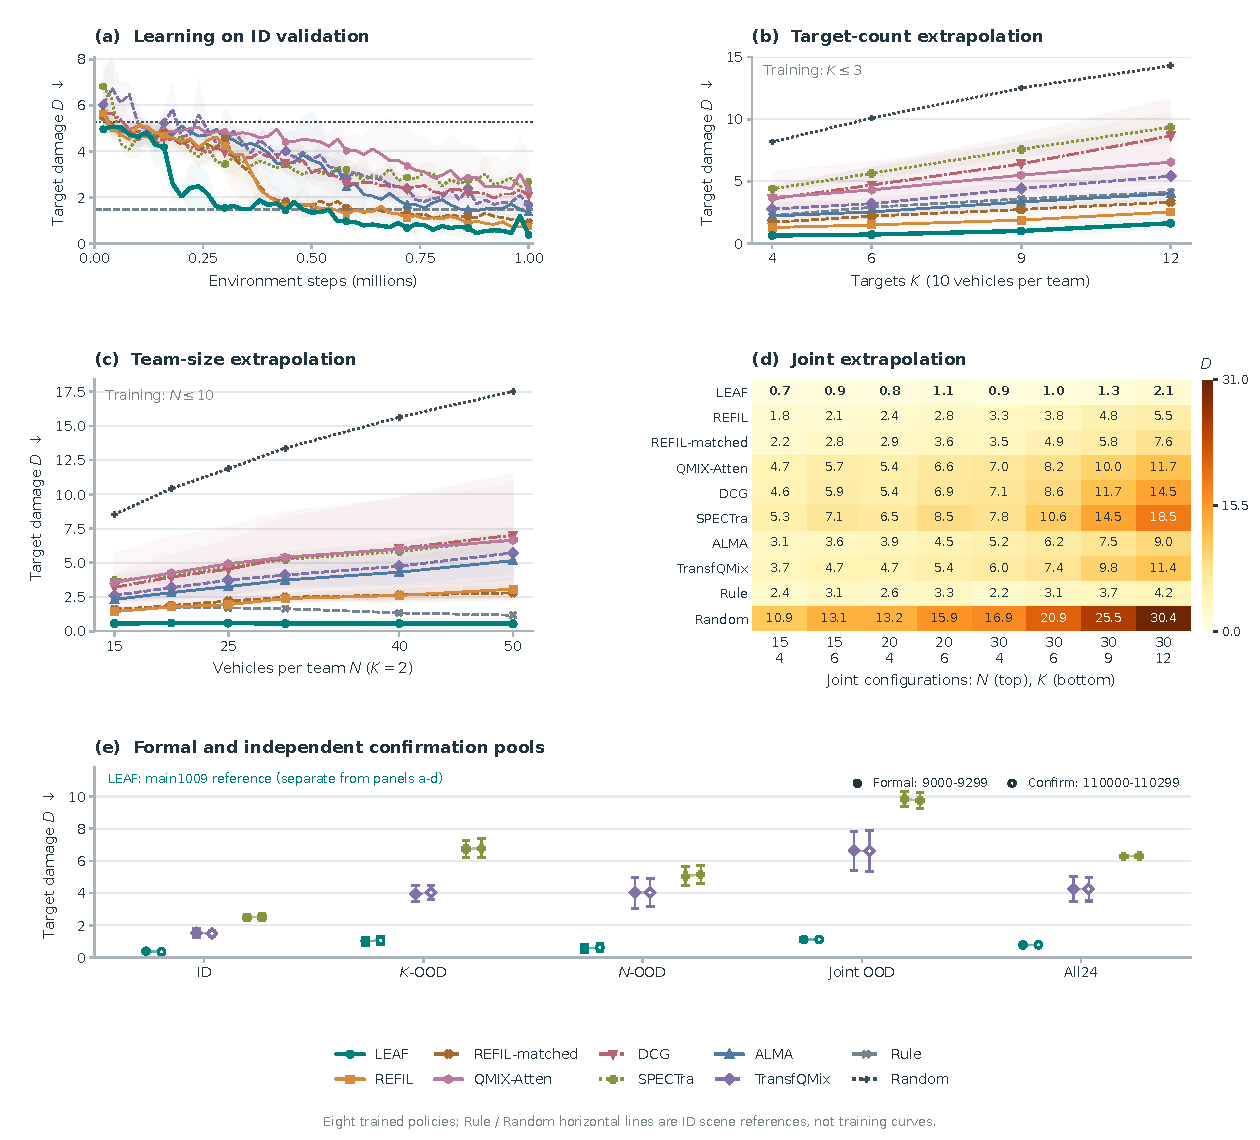
\includegraphics[width=\textwidth]{../Open-SCORE/outputs/main/had/figures/fig_comparison.pdf}
\caption{Eight-method comparison of learning and zero-shot population transfer: LEAF, REFIL, ALMA, TransfQMix, DCG, SPECTra, Rule, and QMIX (the entity-attention adaptation). SPECTra and TransfQMix use the updated input/sampling protocol described in the text. (a) ID validation damage over training. (b)--(c) Frozen-policy damage under target-count and team-size extrapolation. (d) Joint-extrapolation damage. (e) Formal and independent-confirmation All24 damage; LEAF uses the separately recorded depth/confirmation reference pool and does not replace (a)--(d). Learned-method bands show one sample SD across three models; Rule is a formal reference. Table~\ref{tab:had-main} gives the group means and SDs.}
\label{fig:comparison}
\end{figure*}

\subsection{Architecture Design Comparisons}
\label{subsec:ablation}
We decompose LEAF into a context constructor (C), current-self query and reader (Q), stage fusion (F), and host integration with temporal memory (H). Table~\ref{tab:had-core-ablation} maps each historical trained variant to its principal module change; Fig.~\ref{fig:ablation} shows learning and population transfer for LEAF and all seven saved design variants. Saved configurations show that Direct read, Last read, and No host also retain the stopped-gradient history query used by Memory query, whereas LEAF uses a current-self query. They are historical design comparisons, not single-factor ablations of LEAF. Depth-training and parameter-sharing choices are analyzed separately in Section~\ref{subsec:supplement}.

\noindent\textbf{C: context construction before reading.}
\emph{Direct read} bypasses entity updates and reads $H^{(0)}$. Its damage rises from LEAF's $0.405\pm0.097$ to $0.928\pm0.210$ in ID, and from $1.097\pm0.105$ to $3.196\pm0.687$ in Joint OOD, with higher means in the other two groups as well. This trained comparison favors LEAF's combined context-construction and current-self-reading design; its query difference prevents attributing the entire gap to context construction alone. The frozen context interventions below provide complementary evidence of the trained policy's dependence on context.

\noindent\textbf{Q: current-state query with history downstream.}
\emph{Memory query} adds the stopped-gradient previous Temporal GRU hidden state to the query; it retains the reader and temporal network. LEAF's current-self query has lower group mean damage by 0.122, 0.533, 0.424, and 0.849, with three seed pairs favoring LEAF in ID and two in each OOD group. The archived seed-1 pair used six versus twelve parallel collectors (the other runs used twelve), limiting strict attribution to query placement. The result favors the chosen division of information: read the current context, then combine it with temporal history for action selection.

\noindent\textbf{F: access to intermediate stages.}
\emph{Last read} replaces stage fusion with the exit's final read. Its group means are close to LEAF, ranging from $0.434$ versus $0.405$ in ID to $1.269$ versus $1.097$ in Joint OOD. This modest retrained gap, with query history also differing, does not establish an independent benefit from fusion. It is distinct from forcing an already trained LEAF policy to use its last read, which probes dependence on the learned representation in Section~\ref{subsec:mechanism}.

\noindent\textbf{H: integration with cooperative value learning.}
\emph{No host} removes the REFIL attention path, imagined groups, and associated auxiliary loss while retaining a self-projection residual, the relational path, and Temporal GRU. LEAF has lower damage in all four groups, with the largest mean difference, 1.222, in Joint OOD. The removed host package and retained history query prevent assigning this difference to one attention layer or one loss. Temporal memory is retained by every trained variant; its deployment-time role is examined by a frozen reset intervention below.

\HadCoreAblationTable

\begin{figure*}[!t]
\centering
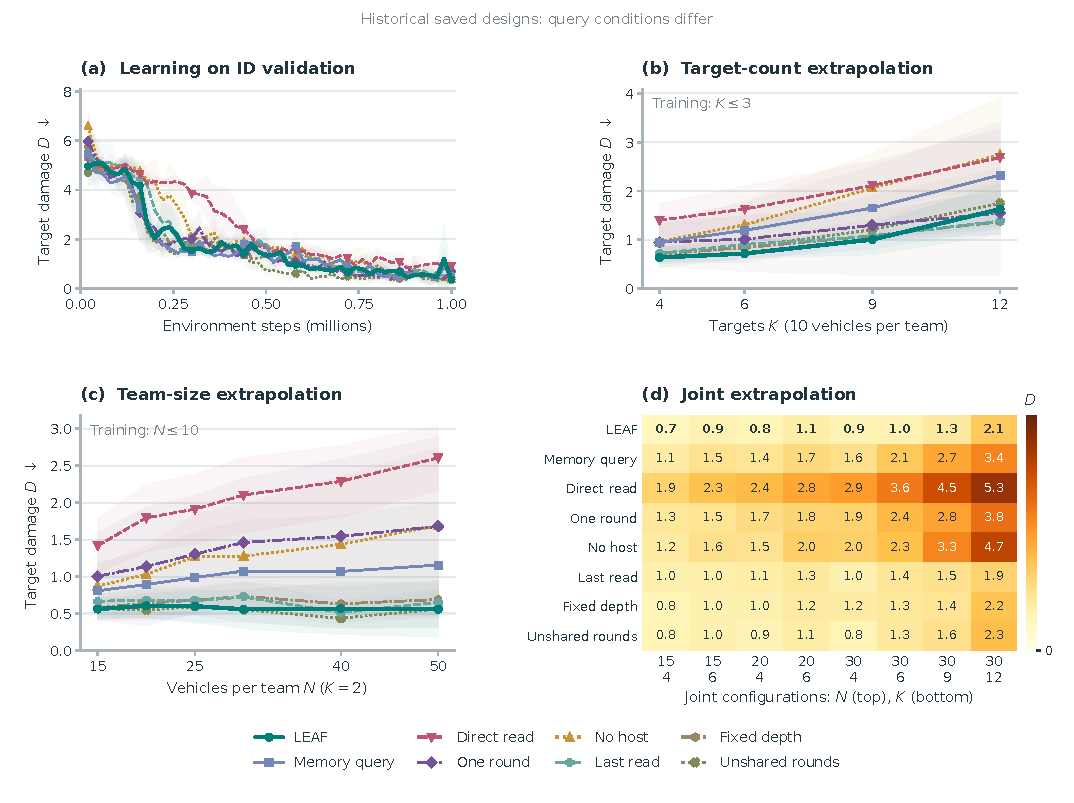
\includegraphics[width=\textwidth]{../Open-SCORE/outputs/main/had/figures/fig_ablation.pdf}
\caption{LEAF and seven saved design variants. (a) ID validation damage over training. (b)--(c) Frozen-policy target-count and team-size transfer. (d) Joint-extrapolation damage. Learned-method bands show one sample SD across three models. The variants retain stopped-gradient history queries, so the contrasts with LEAF are not all single-factor changes. Table~\ref{tab:had-core-ablation} and Table~\ref{tab:had-supplement} give absolute group means and sample SDs.}
\label{fig:ablation}
\end{figure*}

\subsection{Mechanism of Context Use and Reusable Refinement}
\label{subsec:mechanism}
The mechanism study tests three hypotheses implied by the architecture: the trained policy uses constructed current-scene context (H1); receiver-specific intermediate reading works with downstream temporal history (H2); and the learned refinement can be reused across execution depths (H3). The final protection metrics connect these computational observations to the task outcome.

\noindent\textbf{H1: constructed context contributes to the deployed policy.}
Table~\ref{tab:leaf-mechanism} and Fig.~\ref{fig:mechanism}(a) use existing frozen interventions on ten common scenes for each of three models and configurations $(10,10,2)$, $(50,50,2)$, and $(30,30,12)$. Reading the initial $H^{(0)}$ instead of contextualized entities worsens damage in all nine model--configuration pairs. Zeroing the complete relational residual also worsens all nine pairs. In the largest target configuration, their mean damage increases are $32.968\pm8.447$ and $18.788\pm1.144$, respectively. These interventions show that the trained policy uses both contextual processing and its relational feature path. They do not predict how a policy retrained after removal would perform. Each intervention is paired with its runtime-matched local standard, separately from the formal 300-scene pool.

\HadMechanismTable

\begin{figure*}[!t]
\centering
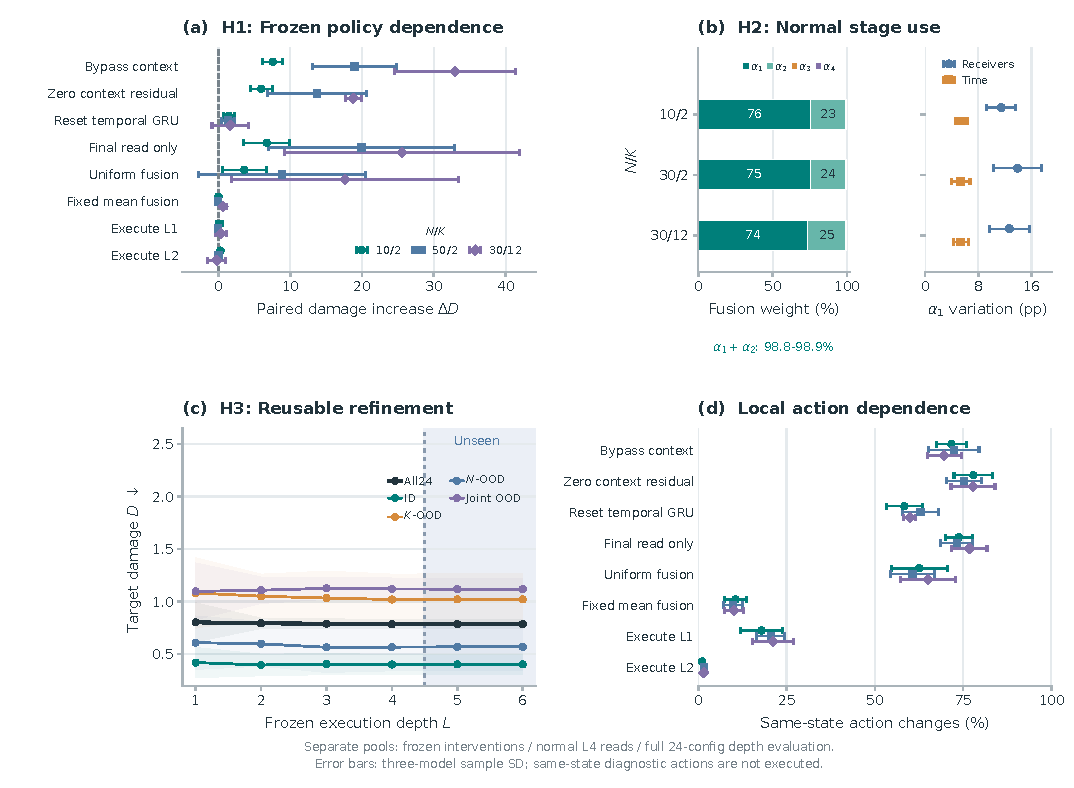
\includegraphics[width=\textwidth]{../Open-SCORE/outputs/main/had/figures/fig_mechanism.pdf}
\caption{Mechanism evidence aligned with the architectural hypotheses. (a) Paired damage changes for eight frozen interventions, including context bypass and zeroing the relational residual. (b) H2: normal R4 fusion weights and receiver/time variation; stacked bars show mean weights. (c) H3: frozen R1--R6 damage; shading marks depths beyond training. Hollow markers give separately trained One round references for $N$-OOD and Joint OOD, with SDs in Table~\ref{tab:had-supplement}. (d) Same-state action-change percentages for the eight interventions; diagnostic actions are not executed and use the same entering temporal state. Error bars/bands show sample SD across three model means. Each panel retains its recorded evaluation pool; Table~\ref{tab:leaf-mechanism} also reports final-read and temporal-reset interventions.}
\label{fig:mechanism}
\end{figure*}

\noindent\textbf{H2: stage reading is receiver-specific, with memory retained downstream.}
Normal R4 records contain 90 episodes and 38,693 live-defender decisions. Three models each execute ten scenes in three configurations: 10v10 with two targets, and 30v30 with two or twelve targets. The first two reads receive $98.909\pm0.265\%$, $98.755\pm0.542\%$, and $98.839\pm0.157\%$ of fusion weight, respectively (Fig.~\ref{fig:mechanism}(b)). Within a physical state, the average SD of the first-round weight across active receivers is 11.44, 13.91, and 12.68 percentage points. Its mean absolute change for the same defender at adjacent steps is 5.49, 5.34, and 5.36 points. Thus receivers sharing an engagement use the stages differently, and those choices evolve over physical time.

Forcing the final read instead of learned fusion worsens all nine model--configuration pairs in Table~\ref{tab:leaf-mechanism}; resetting Temporal GRU every physical step worsens eight of nine. These observations support the division between current-context reading and downstream history in the frozen policy; they do not measure retrained component gains. The roughly 1\% mean omitted fusion mass beyond the two-round prefix is only one factor in Proposition~2. Equation~\eqref{eq:prefix-bound} also involves read displacement; action preservation further depends on downstream sensitivity and the action-value margin. Fusion weights alone are neither causal reward contributions nor a stopping rule; normal R4 computes all four stages.

\noindent\textbf{H3: refinement is reusable across execution depths.}
Figure~\ref{fig:mechanism}(c) executes the same three final LEAF models at R1--R6 on all 24 configurations, with 300 scenes per configuration and exit. R1--R4 are within the training range; R5/R6 extend inference depth without retraining. All24 damage changes from $0.8022\pm0.1849$ at R1 to $0.7845\pm0.0434$ at R4; R5 and R6 remain close, at $0.7851\pm0.0425$ and $0.7849\pm0.0423$. The small paired R2--R4 reduction, 0.008249, has a three-seed 95\% $t$ interval of $[-0.008362,0.024859]$. This is a separately recorded depth-evaluation pool; its R4 values do not replace Table~\ref{tab:had-main}.

The frozen R1 group means in ID, $N$-OOD, and Joint OOD (0.4194, 0.6086, 1.0968) are also below those of the separately trained One round model (0.609, 1.355, 2.157; Table~\ref{tab:had-supplement}). This descriptive, cross-pool comparison shows that useful short execution is compatible with multi-depth training, and the observed advantage does not require executing several rounds at deployment. The One round model also retains a history query; this is not a scene-paired contrast, a single-factor depth-training contrast, or a comparison of equal training computation.

Depth ordering still depends on the configuration. At $(30,30,12)$, R1 has mean damage 1.6378 versus R4's 2.1674; at $(30,30,2)$, R4 has 0.5370 versus R1's 0.6426. Changing depth also changes the reads available to fusion and, through later actions, the temporal states. These closed-loop results support reuse over the evaluated range, not monotonic improvement or arbitrary-depth convergence.



\HadSupplementTable

\begin{figure*}[!t]
\centering
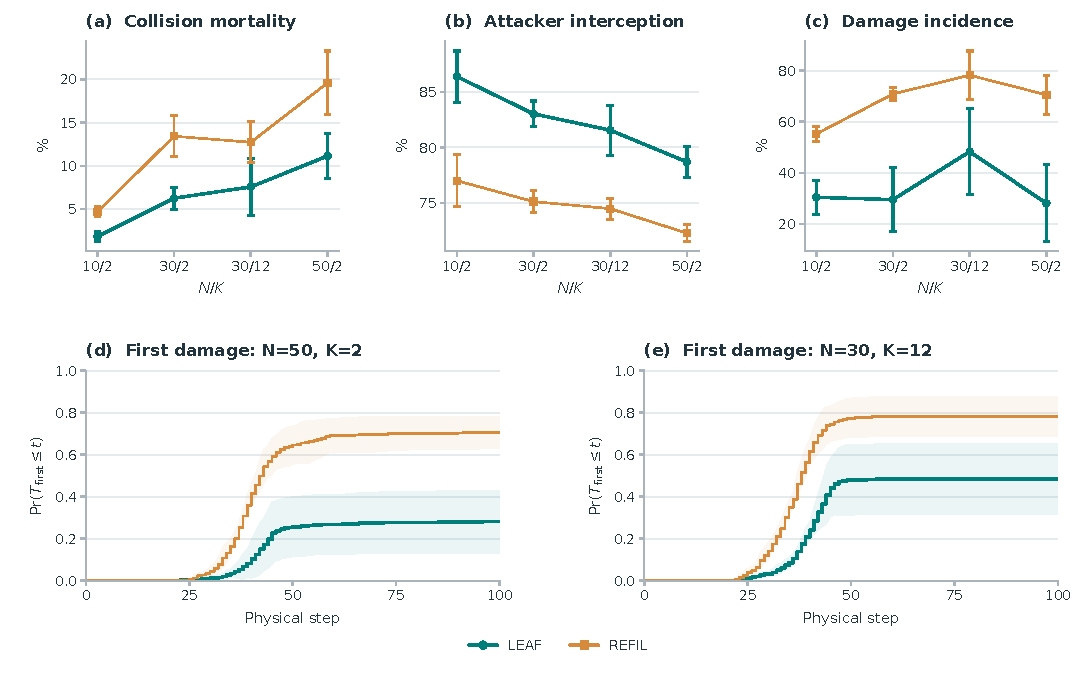
\includegraphics[width=\textwidth]{../Open-SCORE/outputs/main/had/figures/fig_protection.pdf}
\caption{Formal team protection on 300 scenes per configuration. Collision mortality $C$, attacker interception $I$, and target-damage incidence $P$ retain their recorded model-seed means and sample SDs. The first-damage cumulative incidence includes undamaged episodes as non-events rather than dropping them. These formal outcomes are separate from the local frozen and same-state diagnostics in Fig.~\ref{fig:mechanism}.}
\label{fig:protection}
\end{figure*}

\noindent\textbf{From context use to team protection.}
The formal outcomes in Fig.~\ref{fig:protection} return to all 300 scenes per configuration. At $(10,10,2)$, LEAF intercepts $86.38\pm2.31\%$ of attackers versus REFIL's $77.00\pm2.32\%$, while damage incidence falls from $55.22\pm3.10\%$ to $30.44\pm6.74\%$. The same direction holds at $(30,30,2)$ and $(30,30,12)$, despite the different numbers of threatened assets. At $(50,50,2)$, LEAF raises interception to $78.68\pm1.39\%$ from $72.27\pm0.77\%$, reduces collision mortality to $11.14\pm2.63\%$ from $19.59\pm3.69\%$, and reduces damage incidence to $28.11\pm15.03\%$ from $70.56\pm7.65\%$. The representation and recurrent controller thus produce measurable team protection beyond the small training populations.

\subsection{Supplementary Analysis}
\label{subsec:supplement}
The supporting controls in Table~\ref{tab:had-supplement} examine capacity and refinement choices without treating them as additional representation modules.

\noindent\textbf{Capacity control.}
REFIL-matched has 176,393 actor parameters, close to LEAF's 175,754; standard REFIL has 102,025. LEAF retains lower mean damage in all four groups. A comparable parameter budget for the host therefore does not reproduce the protection results, although parameter matching does not establish equal compute cost.

\noindent\textbf{Training depth and parameter sharing.}
\emph{One round} is trained from scratch and executed at R1. Relative to Direct read within the history-query family, one contextual update reduces group mean damage by 0.319, 0.755, 0.665, and 1.039; two of three seed comparisons improve in every group. LEAF further lowers the group means, but that comparison jointly changes query history, depth training, and access to intermediate reads. One round is locally better at $(10,10,12)$, with $D=1.548\pm0.439$ versus LEAF's $1.625\pm0.515$. \emph{Fixed depth} trains at R4 throughout and has group means close to LEAF. \emph{Unshared rounds} uses independent context-update blocks, increasing parameter count, and has lower mean $N$-OOD damage (0.543 versus 0.575). Both also retain history queries. These historical controls characterize design choices; they do not establish a universal independent gain from depth sampling or sharing.


\noindent\textbf{Independent scene confirmation.}
An independent pool of 300 scenes per configuration reuses the frozen models under the archived matched HAD-workbench protocol. All24 damage is $0.7901\pm0.0395$ for LEAF R4, $2.0857\pm0.1905$ for REFIL, $4.2549\pm0.7413$ for the updated TransfQMix, and $6.2964\pm0.0723$ for the updated SPECTra. This corroborates the protection ordering on another scene pool without selecting a new depth. Historical 10-dimensional baseline runs remain archived separately from the updated runs and are not pooled into these means.
